\documentclass[12pt]{article}

\usepackage[margin=1in]{geometry}
\usepackage{amsmath,amsthm,amssymb}
\usepackage{nccmath}
\usepackage{mathtools}
\usepackage{mathrsfs}
\usepackage{enumitem}
\usepackage{physics}
\usepackage{tensor}
\usepackage{subcaption}
\usepackage{pdfpages}
\usepackage{graphicx}
\graphicspath{ {./images/} }

\newcommand{\chrissym}[3]{\Gamma_{#2#3}^#1}

\begin{document}
\title{Homework 7}
\author{Sean Ericson \\ Phys 610}
\maketitle

\section*{Problem 1}
We assume the only change in the physical distance between the test particles is due to the change in the scale factor. In a vacuum dominated universe, the scale factor grows as
\[ a(t) = a_0 e^{Ht},  \]
where $H$ is the Hubble parameter. The physical distance between the test particles is 
\[ d(t) = a(t)r(t), \]
where $r(t)$ is the coordinate separation, which does not change under evolution due only to the scale factor. The physical separation between the particles is then 
\[ d(t) = r_0e^{Ht}. \]
The time for a given relative change in physical separation is therefore
\[ t = H^{-1}\ln(\frac{d}{r_0}). \]
For movement on the order of the initial separation size (i.e. $d \to 2$cm), this is a time scale on the order of $10^{10}$ years. However, if we were able to measure the separation of the particles to the accuracy of LIGO ($\sim 10^{-22}$m), the associated timescale would be on the order of seconds! So, laboratory detection seems like it would be extremely challenging, but not necessarily impossible. 

\section*{Problem 2}
\begin{enumerate}[label=(\alph*)]
    \item Units of physical quantities form a $\mathbb{Q}$-vector space. Let's work in the {Length, Mass, Time} or $\{\mathcal{L}, \mathcal{M}, \mathcal{T}\}$. The units of the constants can then be expressed as
    \[ [c] = \mqty(1\\0\\-1), \quad [\hbar] = \mqty(2\\1\\-1), \quad [G] = \mqty(3\\-1\\2). \]
    Calculating the units of the proposed quantities follows as
    \begin{align*}
        \left[\frac{c^5}{\hbar G^2}\right] &= 5\mqty(1\\0\\-1) - \mqty(2\\1\\-1) - 2\mqty(3\\-1\\2) \\
        &= \mqty(-3\\1\\0) \\
        &= \frac{\mathcal{M}}{\mathcal{L}^3},
    \end{align*}
    and we can see the quantity indeed as units of mass density.

    \item 
    Plugging in the values of the constants and the observed vacuum energy density, we get a ration of $\rho_\Lambda / \rho_\text{Pl} \approx 10^{-123}$, as illustrated in Figure 1.
    \begin{figure}[h]
        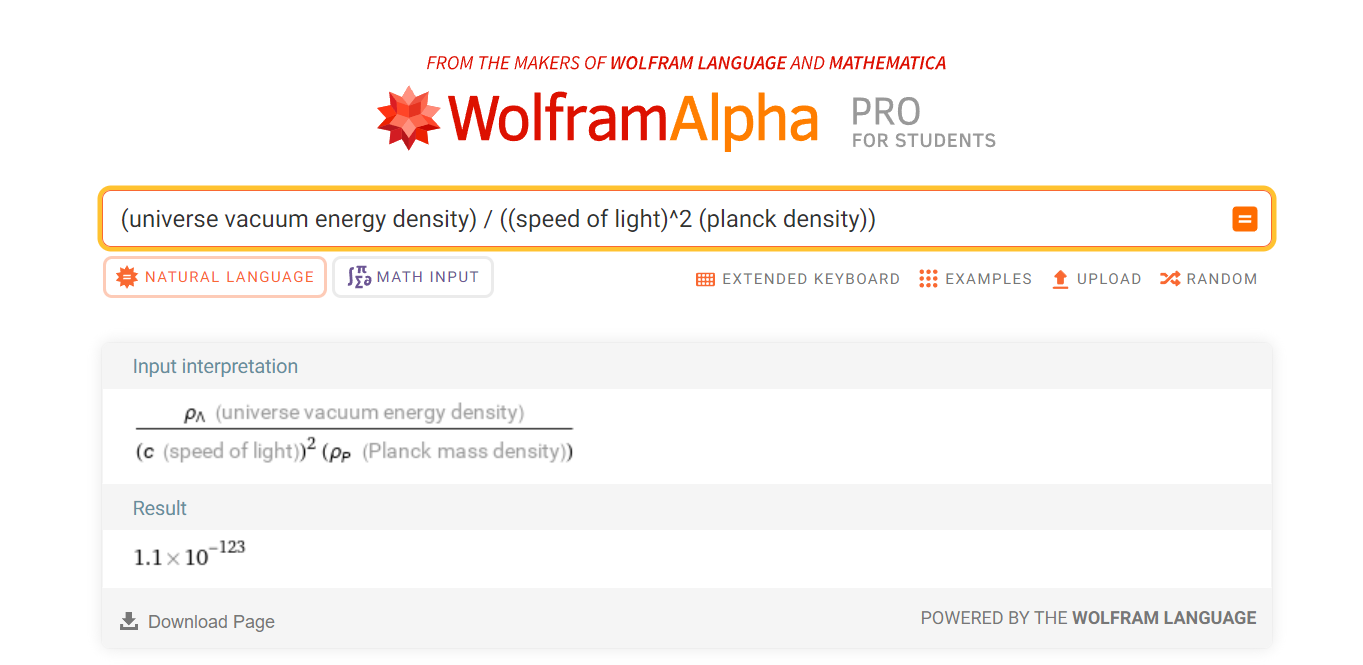
\includegraphics[scale=0.7]{2b.PNG}
        \centering
        \caption{Calculation of $\rho_\Lambda / \rho_\text{Pl}$ via WolframAlpha.}
        \label{fig1}
    \end{figure}


\end{enumerate}


\section*{Problem 3}
\begin{enumerate}[label=(\alph*)]
    \item Matter density is proportional to $a^{-3}$, and the temperature is proportional to $a^{-1}$, so 
    \[ p \propto T\rho \implies \boxed{p \propto a^{-4}} \]

    \item The energy of the neutrinos is proportional to their temperature, and we seek the temperature at which this energy is comparable to their rest mass. Therefore,
    \[ \frac{T}{T_0} \propto \left(\frac{a}{a_0}\right)^{-1} = \frac{a_0}{a} = z + 1 \]
    \[ \implies z \approx \frac{T}{T_0} - 1 \approx \frac{m_\nu}{T_0} - 1 \approx \boxed{579} \]

    \begin{figure}[h]
        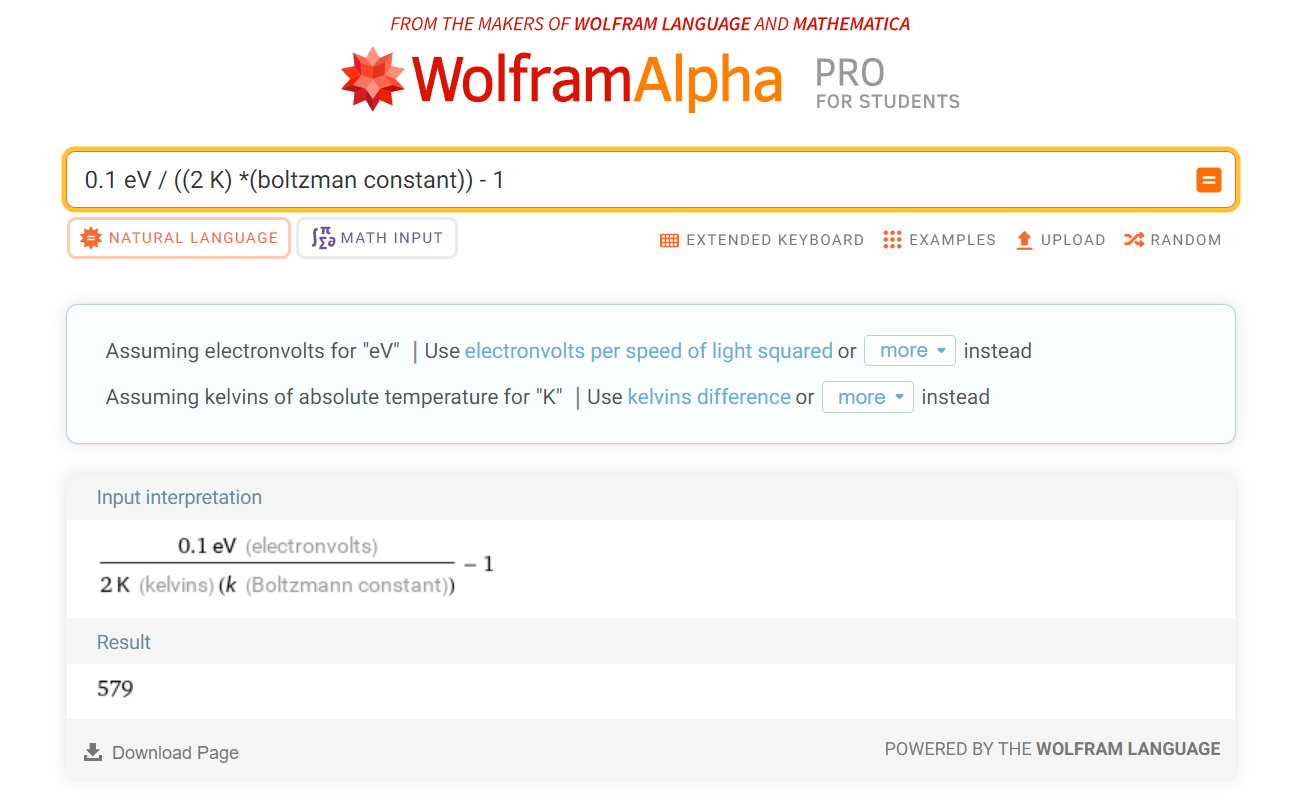
\includegraphics[scale=0.5]{3b.PNG}
        \centering
        \caption{Calculation of $z$ for the neutrino transition via WolframAlpha.}
        \label{fig2}
    \end{figure}
\end{enumerate}


\end{document}